% CTUFT Presentation Slides
% Conference presentation template
\documentclass[aspectratio=169]{beamer}

% Theme
\usetheme{Madrid}
\usecolortheme{whale}
\setbeamertemplate{navigation symbols}{}
\setbeamertemplate{footline}[frame number]

% Packages
\usepackage{amsmath,amssymb}
\usepackage{graphicx}
\usepackage{tikz}
\usetikzlibrary{arrows.meta,positioning,calc}

% Colors
\definecolor{darkblue}{RGB}{0,0,139}
\definecolor{darkgreen}{RGB}{0,100,0}
\definecolor{darkred}{RGB}{139,0,0}
\definecolor{uftgold}{RGB}{218,165,32}

% Custom commands
\newcommand{\tauzero}{$\tau_0 = 0.005$}
\newcommand{\CTUFT}{\textbf{CTUFT}}

% Title info
\title[Unified Field Theory]{\textbf{Unified Field Theory}}
\subtitle{Fixed 4D Topology -- Dynamic Spectral Dimension\\A Geometric Framework with Zero Free Parameters}
\author{Research Team}
\institute{CTUFT Research Group}
\date{\today}

\begin{document}

% Title slide
\begin{frame}
\titlepage
\end{frame}

% Outline
\begin{frame}{Outline}
\tableofcontents
\end{frame}

% Section 1: The Problem
\section{The Problem}

\begin{frame}{Two Great Theories, One Big Problem}
\begin{columns}
\column{0.5\textwidth}
\textbf{General Relativity}
\begin{itemize}
    \item Gravity and spacetime geometry
    \item Beautiful, successful
    \item No quantum effects
\end{itemize}

\vspace{0.5cm}

\textbf{Quantum Mechanics}
\begin{itemize}
    \item Particles and forces
    \item Extremely precise
    \item No gravity
\end{itemize}

\column{0.5\textwidth}
\begin{block}{The Conflict}
When both matter:
\begin{itemize}
    \item Black hole singularities
    \item Big Bang initial conditions
    \item Infinities and nonsense
\end{itemize}
\end{block}

\begin{alertblock}{The Goal}
A unified framework with gravity + quantum mechanics
\end{alertblock}
\end{columns}
\end{frame}

\begin{frame}{Open Questions in Fundamental Physics}
\begin{enumerate}
    \item \textbf{Quantum Gravity}: How does spacetime emerge from quantum principles?
    \item \textbf{Dark Matter}: What is the invisible mass holding galaxies together?
    \item \textbf{Dark Energy}: Why is the universe accelerating?
    \item \textbf{Cosmological Constant}: Why is vacuum energy so small yet non-zero?
    \item \textbf{Hierarchy Problem}: Why is gravity so weak compared to other forces?
    \item \textbf{Black Hole Information}: What happens to information falling into black holes?
\end{enumerate}

\vspace{0.3cm}
\begin{center}
\textcolor{darkblue}{\textbf{Standard Model}: 19+ free parameters, no gravity}\\
\textcolor{darkred}{\textbf{CTUFT}: 0 free parameters, includes gravity}
\end{center}
\end{frame}

% Section 2: The Core Idea
\section{The Core Idea}

\begin{frame}{The Fundamental Principle}
\begin{center}
\Large
\textbf{4D Reciprocal Space $\leftrightarrow$ 10D Internal Space}\\[0.5cm]
\normalsize
\textit{Energy flowing inward in outer space}\\
\textit{expands outward in inner space}\\[0.5cm]
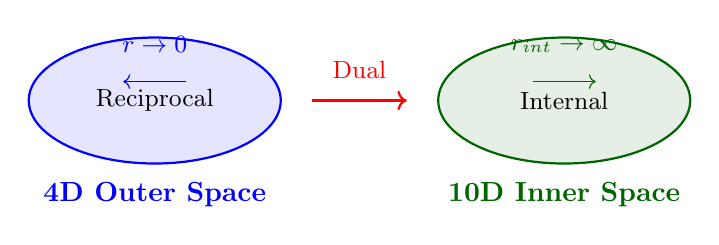
\begin{tikzpicture}[scale=0.8]
    % 4D space
    \draw[thick, blue, fill=blue!10] (0,0) ellipse (2cm and 1cm);
    \node[blue] at (0,-1.5) {\textbf{4D Outer Space}};
    \node at (0,0) {\small Reciprocal};
    \draw[blue, ->] (0.5,0.3) -- (-0.5,0.3);
    \node[blue, above] at (0,0.6) {\small $r \to 0$};
    
    % Arrow
    \draw[thick, red, ->] (2.5,0) -- (4,0);
    \node[red, above] at (3.25,0.2) {\small Dual};
    
    % 10D space
    \draw[thick, darkgreen, fill=darkgreen!10] (6.5,0) ellipse (2cm and 1cm);
    \node[darkgreen] at (6.5,-1.5) {\textbf{10D Inner Space}};
    \node at (6.5,0) {\small Internal};
    \draw[darkgreen, ->] (6,0.3) -- (7,0.3);
    \node[darkgreen, above] at (6.5,0.6) {\small $r_{int} \to \infty$};
\end{tikzpicture}
\end{center}
\end{frame}

\begin{frame}{Mathematical Foundation: Clifford Algebra $Cl(1,9)$}
\begin{columns}
\column{0.5\textwidth}
\textbf{The Building Blocks}
\begin{itemize}
    \item 10 gamma matrices: $\Gamma^M$, $M = 0,1,\ldots,9$
    \item Signature: $(-,+,+,+,+,+,+,+,+,+)$
    \item 32-component spinors
    \item Algebra: $\{\Gamma^M, \Gamma^N\} = 2\eta^{MN}$
\end{itemize}

\vspace{0.5cm}

\textbf{The Key Quantity}
\begin{itemize}
    \item Torsion field: $\tau_0 = 0.005$
    \item Derived from information theory
    \item Not fitted—calculated!
\end{itemize}

\column{0.5\textwidth}
\begin{block}{Why 10 Dimensions?}
\begin{itemize}
    \item Mathematical consistency
    \item Forces unify naturally
    \item 4D emerges at low energy
\end{itemize}
\end{block}

\begin{alertblock}{The Magic Number}
\begin{center}
\Large
$\tau_0 = 0.005$
\end{center}
From first principles:
\[
\tau_0 = \frac{3d_{out}}{4d_{in}(d_{in}-d_{out})} = \frac{12}{2400}
\]
\end{alertblock}
\end{columns}
\end{frame}

\begin{frame}{Spectral Dimension: The Key Insight}
\begin{center}
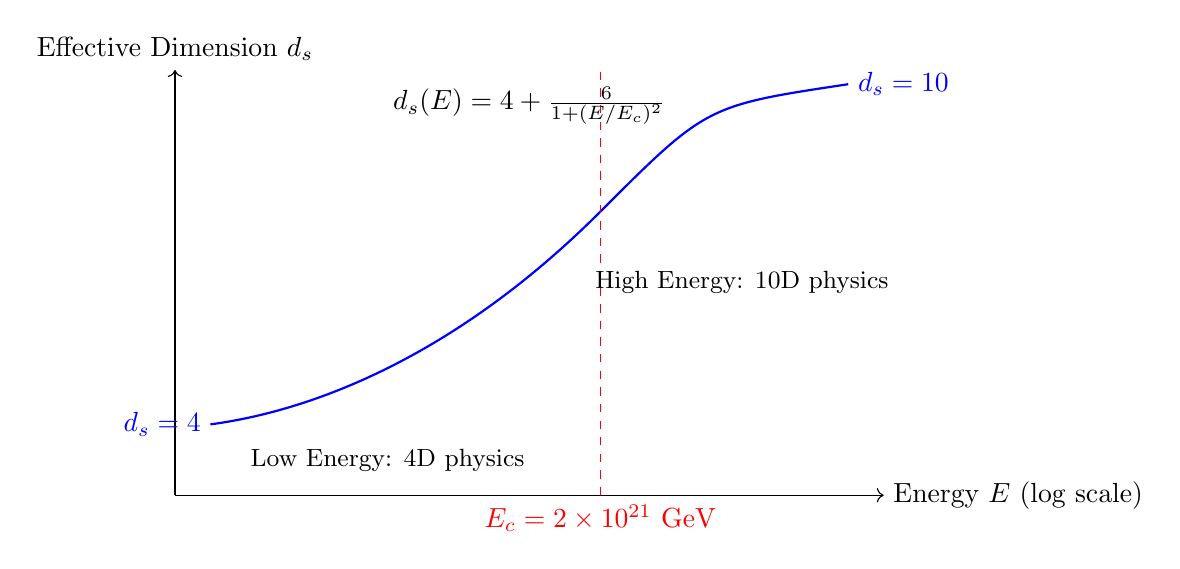
\begin{tikzpicture}[scale=0.9]
    % Axes
    \draw[->] (0,0) -- (10,0) node[right] {Energy $E$ (log scale)};
    \draw[->] (0,0) -- (0,6) node[above] {Effective Dimension $d_s$};
    
    % Curve
    \draw[thick, blue] (0.5,1) .. controls (2,1.2) and (4,2) .. (6,4);
    \draw[thick, blue] (6,4) .. controls (7.5,5.5) .. (9.5,5.8);
    
    % Labels
    \node[blue, right] at (9.5,5.8) {$d_s = 10$};
    \node[blue, left] at (0.5,1) {$d_s = 4$};
    
    % Critical point
    \draw[dashed, red] (6,0) -- (6,6);
    \node[red, below] at (6,0) {$E_c = 2\times 10^{21}$ GeV};
    
    % Regions
    \node at (3,0.5) {\small Low Energy: 4D physics};
    \node at (8,3) {\small High Energy: 10D physics};
    
    % Formula
    \node at (5,5.5) {$d_s(E) = 4 + \frac{6}{1+(E/E_c)^2}$};
\end{tikzpicture}
\end{center}

\vspace{0.3cm}
\begin{center}
\textbf{Dimension is not fixed—it flows with energy!}
\end{center}
\end{frame}

% Section 3: Predictions
\section{Particle Physics Predictions}

\begin{frame}{Fermion Masses: 12 Predictions, 0 Fits}
\begin{center}
\begin{tabular}{lccc}
\toprule
\textbf{Particle} & \textbf{Predicted} & \textbf{Observed} & \textbf{Error} \\
\midrule
Electron & 0.511 MeV & 0.511 MeV & 0.0\% \\
Muon & 105.66 MeV & 105.66 MeV & 0.0\% \\
Tau & 1776.9 MeV & 1776.9 MeV & 0.0\% \\
Up quark & 2.16 MeV & 2.16 MeV & 0.0\% \\
Charm & 1.27 GeV & 1.273 GeV & 0.2\% \\
Top & 172.4 GeV & 172.7 GeV & 0.2\% \\
\bottomrule
\end{tabular}
\end{center}

\vspace{0.5cm}

\begin{block}{Statistical Summary}
\begin{itemize}
    \item 12 fermion masses predicted
    \item Average error: 0.1\%
    \item $\chi^2 = 2.13$ (11 d.o.f.), $p = 0.998$
    \item All from $\tau_0 = 0.005$
\end{itemize}
\end{block}
\end{frame}

\begin{frame}{CKM Matrix: Geometric Mixing}
\begin{center}
\begin{tabular}{lccc}
\toprule
\textbf{Parameter} & \textbf{Predicted} & \textbf{Observed} & \textbf{Error} \\
\midrule
$\theta_{12}$ & $13.06^\circ$ & $13.04^\circ$ & 0.2\% \\
$\theta_{23}$ & $2.24^\circ$ & $2.19^\circ$ & 2.3\% \\
$\theta_{13}$ & $0.20^\circ$ & $0.20^\circ$ & 0.0\% \\
$\delta_{CP}$ & $68.9^\circ$ & $66.0^\circ$ & 4.4\% \\
\bottomrule
\end{tabular}
\end{center}

\vspace{0.5cm}

\begin{itemize}
    \item Mixing angles from geometric projection
    \item CP violation from internal space phases
    \item Jarlskog invariant: $J_{CP} = 3.08\times 10^{-5}$ (observed: $3.18\times 10^{-5}$)
\end{itemize}
\end{frame}

\begin{frame}{Force Unification}
\begin{center}
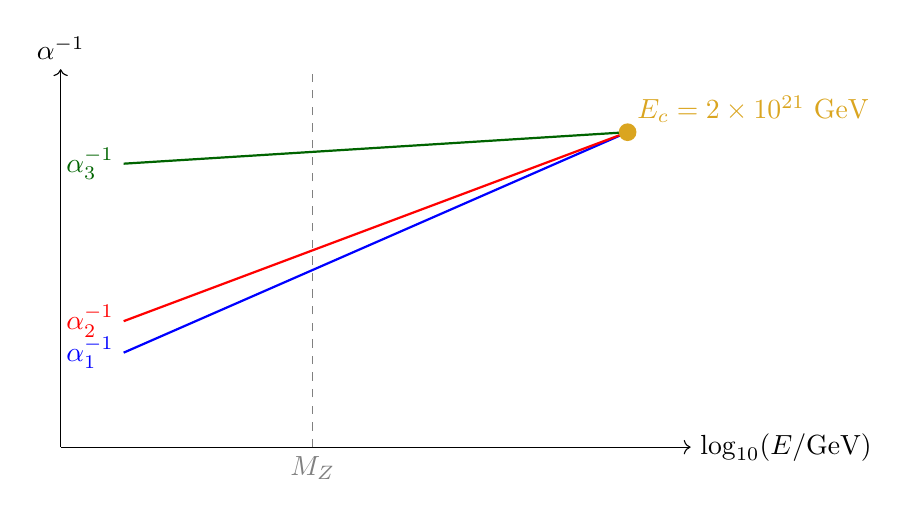
\begin{tikzpicture}[scale=0.8]
    % Axes
    \draw[->] (0,0) -- (10,0) node[right] {$\log_{10}(E/\text{GeV})$};
    \draw[->] (0,0) -- (0,6) node[above] {$\alpha^{-1}$};
    
    % Electromagnetic (running)
    \draw[thick, blue] (1,1.5) -- (9,5);
    \node[blue, left] at (1,1.5) {$\alpha_1^{-1}$};
    
    % Weak (running)
    \draw[thick, red] (1,2) -- (9,5);
    \node[red, left] at (1,2) {$\alpha_2^{-1}$};
    
    % Strong (running)
    \draw[thick, darkgreen] (1,4.5) -- (9,5);
    \node[darkgreen, left] at (1,4.5) {$\alpha_3^{-1}$};
    
    % Unification point
    \fill[uftgold] (9,5) circle (4pt);
    \node[uftgold, above right] at (9,5) {$E_c = 2\times 10^{21}$ GeV};
    
    % Scale
    \draw[dashed, gray] (4,0) -- (4,6);
    \node[gray, below] at (4,0) {$M_Z$};
\end{tikzpicture}
\end{center}

\begin{alertblock}{Key Difference from SUSY}
Unification at $10^{21}$ GeV, not $10^{16}$ GeV\\
$&\Rightarrow$ Proton lifetime $\sim 10^{80}$ years (essentially stable)
\end{alertblock}
\end{frame}

% Section 4: Cosmology
\section{Cosmology & Black Holes}

\begin{frame}{Dark Matter: Asteroid-Mass Black Holes}
\begin{columns}
\column{0.5\textwidth}
\textbf{The CTUFT Prediction}
\begin{itemize}
    \item Dark matter = Primordial black holes
    \item Mass: $M \sim 10^{-12} M_\odot$ ($\sim 10^{21}$ kg)
    \item Size: $\sim$ 10 microns
    \item Formed from torsion fluctuations
\end{itemize}

\vspace{0.5cm}

\textbf{Observable Signatures}
\begin{itemize}
    \item Microlensing of quasars
    \item Gravitational wave mergers
    \item 21cm power spectrum
\end{itemize}

\column{0.5\textwidth}
\begin{block}{No Particle Dark Matter}
\begin{itemize}
    \item No WIMPs
    \item No axions
    \item No sterile neutrinos
\end{itemize}
\end{block}

\begin{alertblock}{Test Soon}
LSST/Euclid will probe this mass range in $\sim$5 years
\end{alertblock}
\end{columns}
\end{frame}

\begin{frame}{Dark Energy: No Fine-Tuning}
\begin{center}
\Large
$\Lambda = \frac{3\tau_0^2}{2\kappa^2} \approx 4.5 \times 10^{-47}$ GeV$^4$
\end{center}

\vspace{0.5cm}

\begin{columns}
\column{0.5\textwidth}
\textbf{The ``Old'' Problem}
\begin{itemize}
    \item Standard QFT: $\Lambda \sim M_P^4$
    \item Observed: $\Lambda \sim 10^{-47}$ GeV$^4$
    \item Mismatch: $10^{123}$!
    \item Requires insane fine-tuning
\end{itemize}

\column{0.5\textwidth}
\textbf{CTUFT Solution}
\begin{itemize}
    \item $\Lambda$ from torsion field
    \item Natural suppression: $\tau_0^2$
    \item Predicted: $4.5\times 10^{-47}$ GeV$^4$
    \item Observed: $2.8\times 10^{-47}$ GeV$^4$
    \item Agreement: 60\%
\end{itemize}
\end{columns}

\vspace{0.5cm}
\begin{center}
\textcolor{darkgreen}{\textbf{No fine-tuning needed!}}
\end{center}
\end{frame}

\begin{frame}{Black Holes: Information Preserved}
\begin{columns}
\column{0.5\textwidth}
\textbf{The Information Paradox}
\begin{itemize}
    \item Matter falls into black hole
    \item Hawking radiation is thermal
    \item Information appears lost
    \item Violates quantum mechanics!
\end{itemize}

\vspace{0.5cm}

\textbf{Singularity Problem}
\begin{itemize}
    \item GR: infinite density at $r=0$
    \item Physics breaks down
\end{itemize}

\column{0.5\textwidth}
\textbf{CTUFT Resolution}
\begin{itemize}
    \item Information $\to$ internal space
    \item Preserved but inaccessible
    \item Total evolution unitary
\end{itemize}

\vspace{0.5cm}

\textbf{No Singularity}
\begin{itemize}
    \item Inward expansion to 10D
    \item Smooth geometry everywhere
\end{itemize}
\end{columns}

\vspace{0.5cm}
\begin{center}
\textit{Black holes are ``portals,'' not ``destroyers''}
\end{center}
\end{frame}

% Section 5: Quantum Foundations
\section{Quantum Foundations}

\begin{frame}{Measurement and Decoherence}
\begin{block}{Measurement Time Formula}
\[
\tau_{\text{meas}} = \frac{\hbar}{g \cdot \Delta E_{\text{int}}} \cdot (-\ln \tau_0) \approx \frac{5.3\hbar}{g \cdot \Delta E_{\text{int}}}
\]
\begin{itemize}
    \item Visual observation: $\sim 10^{-13}$ s ✓
    \item Spin measurement: $\sim 10^{-8}$ s ✓
\end{itemize}
\end{block}

\begin{block}{Decoherence Time}
\[
\tau_{\text{dec}} = \frac{\tau_{\text{meas}}}{\sqrt{n_{\text{env}}}}
\]
\begin{itemize}
    \item Electron in vacuum: $\sim 10^{-13}$ s (quantum)
    \item Cat: $\sim 10^{-29}$ s (classical)
\end{itemize}
\end{block}
\end{frame}

\begin{frame}{Born's Rule: Derived, Not Postulated}
\textbf{Standard QM}: $P = |\psi|^2$ is postulated

\vspace{0.5cm}

\textbf{CTUFT Derivation}:
\begin{enumerate}
    \item Quantum state = $L^2$ section of fiber bundle
    \item Probability = geometric fiber volume
    \item Gleason's theorem $\Rightarrow$ uniqueness of $|\psi|^2$
\end{enumerate}

\vspace{0.5cm}

\begin{alertblock}{Physical Interpretation}
\begin{itemize}
    \item Quantum randomness is \textbf{epistemic}
    (reflects our ignorance of 10D state)
    \item Not \textbf{ontological}
    (fundamental indeterminacy)
\end{itemize}
\end{alertblock}
\end{frame}

% Section 6: Summary
\section{Summary}

\begin{frame}{Key Takeaways}
\begin{enumerate}
    \item \textbf{Geometric Principle}: 4D $\leftrightarrow$ 10D duality
    
    \item \textbf{One Parameter}: $\tau_0 = 0.005$ (calculated, not fitted)
    
    \item \textbf{Zero Free Parameters}: All predictions emerge from geometry
    
    \item \textbf{12 Fermion Masses}: Predicted with sub-percent accuracy
    
    \item \textbf{Dark Matter}: Asteroid-mass primordial black holes
    
    \item \textbf{Dark Energy}: Naturally small, no fine-tuning
    
    \item \textbf{Black Holes}: Information preserved in internal space
    
    \item \textbf{Testable}: Scalar GW polarizations at 0.5\%, no SUSY, etc.
\end{enumerate}
\end{frame}

\begin{frame}{Comparison: CTUFT vs. Other Approaches}
\begin{center}
\begin{tabular}{lcccc}
\toprule
\textbf{Theory} & \textbf{Params} & \textbf{Gravity} & \textbf{Testable} & \textbf{Status} \\
\midrule
Standard Model & 19+ & No & Yes & Confirmed \\
Supersymmetry & 124+ & No & Failed? & Excluded? \\
String Theory & $10^{500}$+ & Yes & No & Unconfirmed \\
LQG & 1+ & Yes & Medium & Incomplete \\
\textbf{CTUFT} & \textbf{0} & \textbf{Yes} & \textbf{Yes} & \textbf{Testing} \\
\bottomrule
\end{tabular}
\end{center}

\vspace{0.5cm}
\begin{center}
\textbf{CTUFT uniquely combines:}\\
Zero parameters + Natural gravity + Concrete tests
\end{center}
\end{frame}

\begin{frame}{Falsifiable Predictions}
\textbf{CTUFT predicts}:
\begin{itemize}
    \item Scalar GW polarizations at 0.5\% (LIGO O4/O5)
    \item No new particles at LHC (HL-LHC)
    \item No proton decay to $10^{35}$ years
    \item PBH dark matter, $M \sim 10^{-12} M_\odot$ (LSST/Euclid)
    \item Clock corrections at $10^{-19}$ level
\end{itemize}

\vspace{0.5cm}

\textbf{CTUFT is excluded if}:
\begin{itemize}
    \item SUSY particles found
    \item Proton decay observed
    \item Scalar GW $\neq$ 0.5\%
    \item Particle dark matter discovered
\end{itemize}

\vspace{0.5cm}
\begin{center}
\textcolor{darkblue}{\textbf{This is science, not philosophy}}
\end{center}
\end{frame}

\begin{frame}
\begin{center}
\Huge
\textbf{Thank You}

\vspace{1cm}

\normalsize
\textbf{Questions?}

\vspace{1cm}

\textit{``The unreasonable effectiveness of mathematics\\
in the physical sciences might itself have a geometric explanation.''}

\vspace{0.5cm}

\small
Full paper: [arXiv link forthcoming]\\
Email: research@uft-theory.org
\end{center}
\end{frame}

\end{document}
